\section{Auswertung}
\label{sec:Auswertung}
In diesem Abschnitt werden nun die Messungen zur Koinzidenzschaltung, zur Kalibrierung des MCA und letztendlich zur Bestimmung der Lebensdauer der kosmischen Myonen ausgewertet.
Alle erstellten Grafiken und Rechnungen werden mit Python \cite{python} durchgeführt.
\subsection{Bestimmung der Auflösung}
Im ersten Teil werden die drei durchgeführten Messungen zur Bestimmun der Auflösung analysiert. Zunächst wird eine Pulsbreite von $t_\mathrm{1}=\SI{20}{\second}$ betrachtet.
Die aufgenommenen Messdaten finden sich in Tabelle \ref{tab:tab1}. Die Fehler der Counts $N$ sind durch $\sqrt{N}$ gegeben.
\begin{table}
  \centering
  \caption{Messdaten für eine Pulsbreite von $t_\mathrm{1}=\SI{20}{\second}$.}
  \label{tab:tab1}
  \begin{tabular}{c c}
    \toprule
		$\Delta t\, / \, \SI{}{\nano\second}$ & $\mathrm{Counts} \, N$ \\
    \midrule
    -24 & $12\pm3.5$ \\
		-22 & $32\pm5.7$ \\
		-20 & $56\pm7.5$ \\
		-18 & $71\pm8.4$ \\
		-16 & $123\pm11.1$ \\
		-14 & $157\pm12.5$ \\
		-12 & $167\pm13.0$ \\
		-10 & $180\pm13.4$ \\
		-8 & $199\pm14.1$ \\
		-6 & $183\pm13.5$ \\
		-4 & $192\pm13.9$ \\
		-2 & $196\pm14.0$ \\
		0  & $212\pm14.6$ \\
		2 & $218\pm14.8$ \\
		4 & $207\pm14.4$ \\
		6 & $188\pm13.7$ \\
		8 & $188\pm13.7$ \\
		10 & $187\pm13.7$ \\
		12 & $183\pm13.5$ \\
		14 & $179\pm13.4$ \\
		16 & $142\pm11.9$ \\
		18 & $137\pm11.7$ \\
		20 & $122\pm11.0$ \\
		22 & $103\pm10.1$ \\
		24 & $91\pm9.5$ \\
		26 & $64\pm8$ \\
		28 & $36\pm6$ \\
    \bottomrule
  \end{tabular}
\end{table}
\FloatBarrier
\noindent In Abbildung (\ref{fig:plateau1}) sind die Messdaten graphisch dargestellt.
\begin{figure}
	\centering
	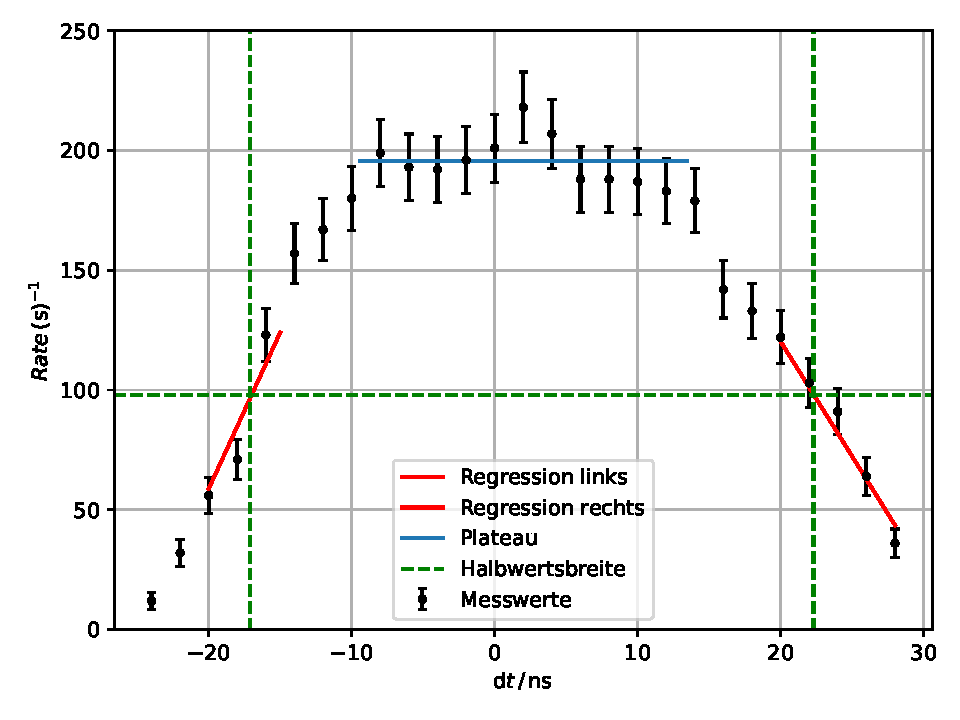
\includegraphics[scale=0.7]{fig/Plateau.pdf}
	\caption{Graphische Darstellung der Messdaten zur Bestimmung der Auflösung.}
	\label{fig:plateau1}
\end{figure}
\FloatBarrier
\noindent An den beiden vertikalen gestrichelten Linien wird die Halbswertsbreite ausgelesen zu:
\begin{align*}
	\Delta t_\mathrm{links}&=\SI{17.5}{\nano\second} \\
	\Delta t_\mathrm{rechts}&=\SI{22.3}{\nano\second} \\
\end{align*}
Daraus folgt für eine Pulsbreite von $t_\mathrm{1}=\SI{20}{\nano\second}$ eine Halbswertsbreite von $t_\mathrm{HWZ}=\SI{39.8}{\nano\second}$. Daraus ergibt sich eine Auflösung von:
\begin{align*}
	t_\mathrm{Auflösung}&=2 t_\mathrm{1}-t_\mathrm{HWZ} \\
	t_\mathrm{Auflösung}&=\SI{0.2}{\nano\second}
\end{align*}
Als nächstes wird nun die Pulsbreite von $t_\mathrm{2}=\SI{15}{\nano\second}$ betrachtet. Die Daten finden sich in Tabelle \ref{tab:tab2}:
\begin{table}
  \centering
  \caption{Messdaten für eine Pulsbreite von $t_\mathrm{2}=\SI{15}{\second}$.}
  \label{tab:tab2}
  \begin{tabular}{c c}
    \toprule
		$\Delta t\, / \, \SI{}{\nano\second}$ & $\mathrm{Counts} \, N$ \\
    \midrule
		-14 & $7\pm2.6$ \\
		-12 & $25\pm5.0$ \\
		-10 & $40\pm6.3$ \\
		-8 & $49\pm7.0$ \\
		-6 & $113\pm10.6$ \\
		-4 & $153\pm12.4$ \\
		-2 & $167\pm12.9$ \\
		0  & $205\pm14.3$ \\
		2 & $212\pm14.6$ \\
		4 & $216\pm14.7$ \\
		6 & $214\pm14.6$ \\
		8 & $199\pm14.1$ \\
		10 & $194\pm13.9$ \\
		12 & $192\pm13.9$ \\
		14 & $151\pm12.3$ \\
		16 & $129\pm11.4$ \\
		18 & $119\pm10.9$ \\
		20 & $70\pm8.4$ \\
		22 & $39\pm6.2$ \\
		24 & $16\pm4.0$ \\
    \bottomrule
  \end{tabular}
\end{table}
\FloatBarrier
\noindent In Abbildung (\ref{fig:plateau2}) sind die Messdaten graphisch dargestellt.
\begin{figure}
	\centering
	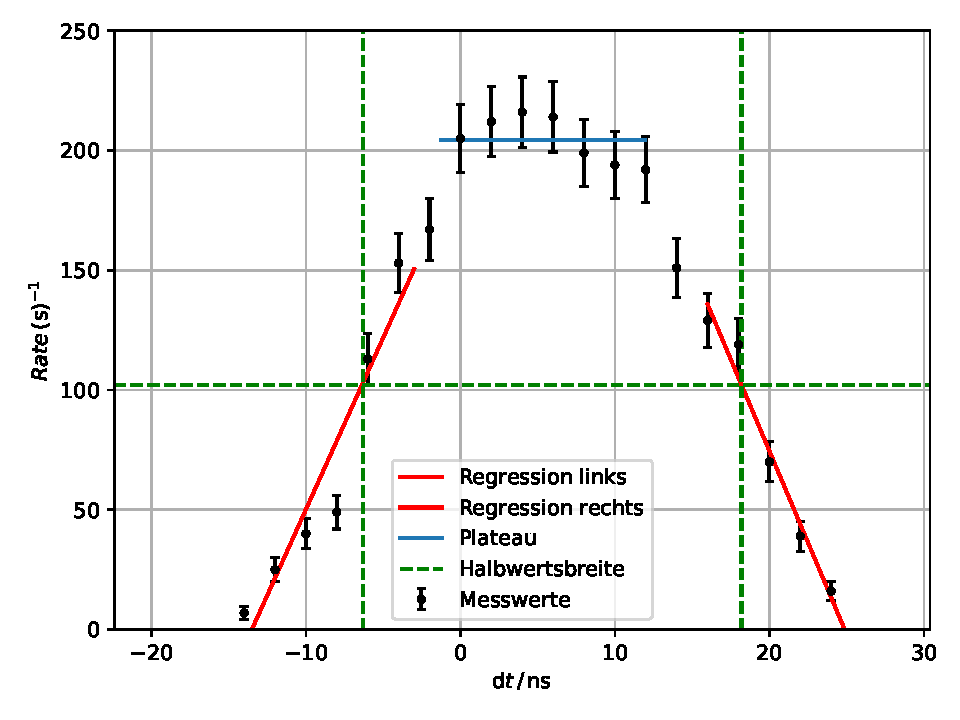
\includegraphics[scale=0.7]{fig/Plateau2.pdf}
	\caption{Graphische Darstellung der Messdaten zur Bestimmung der Auflösung.}
	\label{fig:plateau2}
\end{figure}
\FloatBarrier
\noindent An den beiden vertikalen gestrichelten Linien wird die Halbswertsbreite ausgelesen zu:
\begin{align*}
	\Delta t_\mathrm{links}&=\SI{5.4}{\nano\second} \\
	\Delta t_\mathrm{rechts}&=\SI{18.2}{\nano\second} \\
\end{align*}
Daraus folgt für eine Pulsbreite von $t_\mathrm{2}=\SI{15}{\nano\second}$ eine Halbswertsbreite von $t_\mathrm{HWZ}=\SI{23.6}{\nano\second}$. Daraus ergibt sich eine Auflösung von:
\begin{align*}
	t_\mathrm{Auflösung}&=2 t_\mathrm{2}-t_\mathrm{HWZ} \\
	t_\mathrm{Auflösung}&=\SI{6.4}{\nano\second}
\end{align*}
Als letztes wird nun noch die letzte Pulsbreite von $t_\mathrm{3}=\SI{10}{\nano\second}$ betrachtet. Die aufgenommenen Messdaten finden sich in Tabelle \ref{tab:tab3}:
\begin{table}
  \centering
  \caption{Messdaten für eine Pulsbreite von $t_\mathrm{3}=\SI{10}{\second}$.}
  \label{tab:tab3}
  \begin{tabular}{c c}
    \toprule
		$\Delta t\, / \, \SI{}{\nano\second}$ & $\mathrm{Counts} \, N$ \\
    \midrule
    -7 & $5\pm2.2$ \\
		-6 & $13\pm3.6$ \\
		-5 & $31\pm5.6$ \\
		-4 & $38\pm6.2$ \\
		-3 & $60\pm7.7$ \\
		-2 & $63\pm7.9$ \\
		-1 & $84\pm9.2$ \\
		0 & $110\pm10.5$ \\
		1 & $119\pm10.9$ \\
		2 & $126\pm11.2$ \\
		3 & $145\pm12.0$ \\
		4 & $144\pm12.0$ \\
		5 & $163\pm12.8$ \\
		6 & $150\pm12.2$ \\
		7 & $161\pm12.7$ \\
		8 & $160\pm12.6$ \\
		9 & $162\pm12.7$ \\
		10 & $132\pm11.5$ \\
		11 & $133\pm11.5$ \\
		12 & $122\pm11.0$ \\
		13 & $119\pm10.9$ \\
		14 & $90\pm9.5$ \\
		15 & $85\pm9.2$ \\
		16 & $59\pm7.7$ \\
		17 & $46\pm6.8$ \\
		18 & $14\pm3.7$ \\
		19 & $6\pm2.5$ \\
    \bottomrule
  \end{tabular}
\end{table}
\FloatBarrier
\noindent In Abbildung (\ref{fig:plateau3}) sind die Messdaten graphisch dargestellt.
\begin{figure}
	\centering
	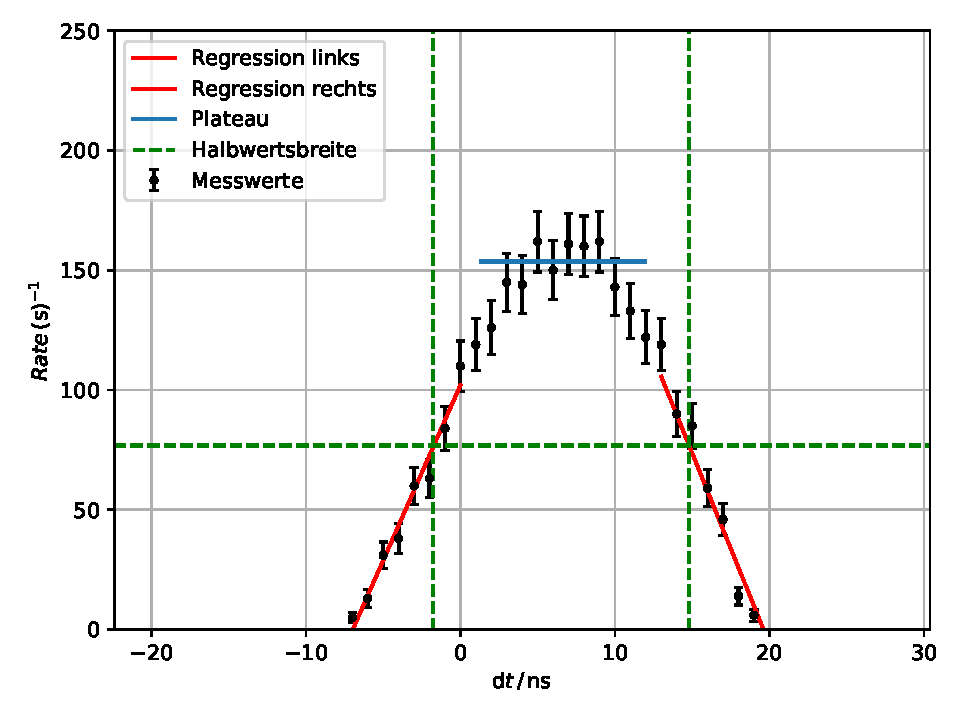
\includegraphics[scale=0.7]{fig/Plateau3.pdf}
	\caption{Graphische Darstellung der Messdaten zur Bestimmung der Auflösung.}
	\label{fig:plateau3}
\end{figure}
\FloatBarrier
\noindent An den beiden vertikalen gestrichelten Linien wird die Halbswertsbreite ausgelesen zu:
\begin{align*}
	\Delta t_\mathrm{links}&=\SI{1.75}{\nano\second} \\
	\Delta t_\mathrm{rechts}&=\SI{14.8}{\nano\second} \\
\end{align*}
Daraus folgt für eine Pulsbreite von $t_\mathrm{3}=\SI{10}{\nano\second}$ eine Halbswertsbreite von $t_\mathrm{HWZ}=\SI{16.55}{\nano\second}$. Daraus ergibt sich eine Auflösung von:
\begin{align*}
	t_\mathrm{Auflösung}&=2 t_\mathrm{3}-t_\mathrm{HWZ} \\
	t_\mathrm{Auflösung}&=\SI{3.45}{\nano\second}
\end{align*}
\subsection{Kalibrierung des MCA}
In diesem Teil der Auswertung wird der MCA kalibriert. In Tabelle \ref{tab:tab4} sind die Messdaten dargestellt.
\begin{table}
  \centering
  \caption{Messdaten für die Kalibrierung des MCA.}
  \label{tab:tab4}
  \begin{tabular}{c c}
    \toprule
		$\mathrm{Kanalnummer}$ & $\Delta t\, / \, \SI{}{\micro\second}$ \\
    \midrule
		37 & 0.8 \\
		81 & 1.8 \\
		126 & 2.8 \\
		171 & 3.8 \\
		216 & 4.8 \\
		261 & 5.8 \\
		306 & 6.8 \\
		350 & 7.8 \\
		395 & 8.8 \\
		440 & 9.8 \\
    \bottomrule
  \end{tabular}
\end{table}
\FloatBarrier
\noindent Nun wird eine Ausgleichsrechnung der Form:
\begin{align*}
	T_\mathrm{VZ}=m\cdot \mathrm{Kanalnummer} + n
\end{align*}
Dabei ergeben sich die Parameter:
\begin{align*}
	m &= \SI{0.02231(1)}{\micro\second} \, \mathrm{pro} \, \mathrm{Kanal} \\
	n &= \SI{-0.017(5)}{\micro\second}
\end{align*}
Dadurch ist es möglich die x-Achse nun mit Zeit anstatt den Kanalnummern skaliert. In Abbildung (\ref{fig:Kanal}) ist dies graphisch dargestellt:
\begin{figure}
	\centering
	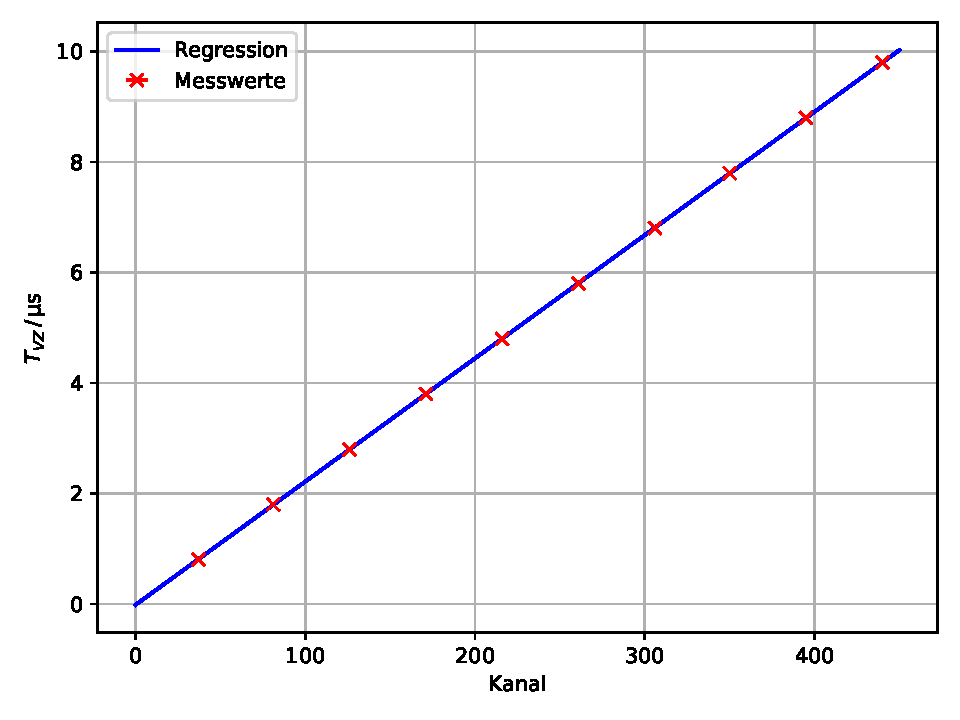
\includegraphics[scale=0.7]{fig/Kanal.pdf}
	\caption{Graphische Darstellung der Messdaten zur Kalibrierung des MCA.}
	\label{fig:Kanal}
\end{figure}
\FloatBarrier
\subsection{Bestimmung der Lebensdauer}
Für die Langzeitmessung sind in einer Messzeit von $t_\mathrm{Mess}=\SI{272190}{\second}$ $N=3256768$ Startimuplse registriert worden.
Aus diesen wird eine Ausgleichsrechnung der Form
\begin{equation}
	N(t)=N_\mathrm{0} \exp(-\lambda t) + U
\end{equation}
durchgeführt. In Abbildung (\ref{fig:spekt}) ist diese Funktion dargestellt:
\begin{figure}
	\centering
	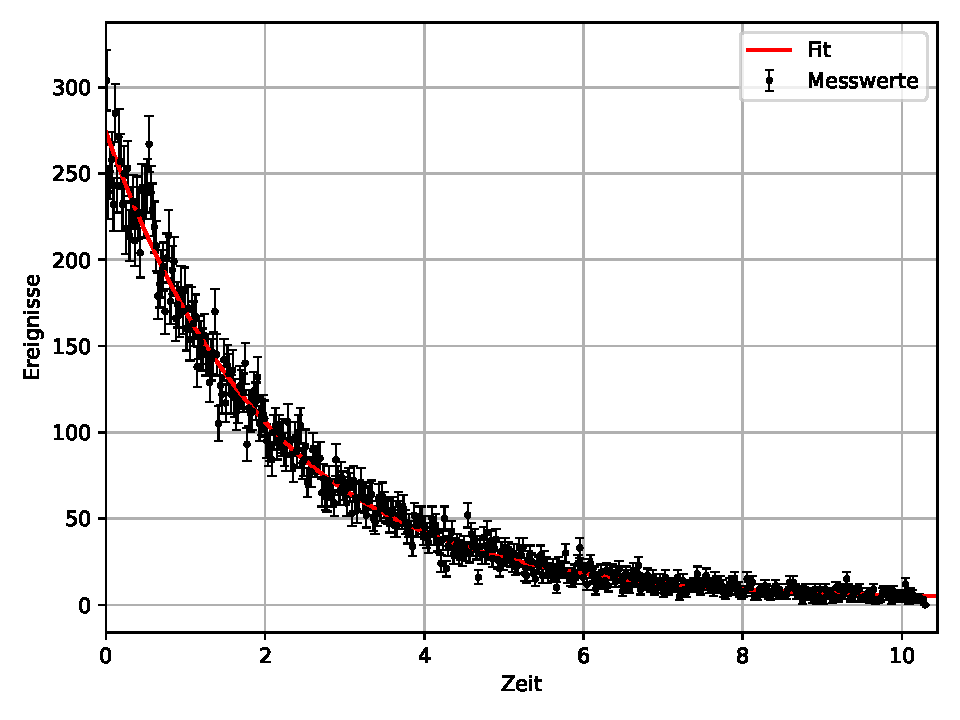
\includegraphics[scale=0.7]{fig/spektrum1_fit.pdf}
	\caption{Graphische Darstellung der Ergebnisse zur Langzeitmessung für die Lebensdauer der Myonen.}
	\label{fig:spekt}
\end{figure}
\FloatBarrier
\noindent Daraus ergeben sich die folgenden Parameter:
\begin{align*}
	N_\mathrm{0} &= 270.6\pm1 \\
	\lambda &= \SI{0.486(7)}{1\per\micro\second} \\
	U_\mathrm{Fit} &= 3.4\pm0.8 \, \dfrac{\mathrm{Counts}}{\mathrm{Kanal}}
\end{align*}
Die Lebensdauer berechet sich nach Gleichung (\ref{eqn:Erwa}) zu:
\begin{align*}
	\tau = \SI{2.06(3)}{\micro\second}
\end{align*}
Zu beachten ist das einige Kanäle nicht berücksichtigt wurden für die Ausgleichsrechnung. Dabei handelt es sich um die ersten drei Kanäle sowie alle Kanäle mit einer Kanalnummer von 465 oder höher, da dort eine Zählrate von Null vorliegt.
\subsection{Bestimmung des Untergrunds}
Zusätzlich zu dem Wert $U_\mathrm{Fit}=3.4\pm0.8$ gibt es eine weitere Möglichkeit den Untergrund zu bestimmen. Dies geschieht mithilfe der Annahme einer Poissonverteilung für den Eintritt eines zusätzlichen Myons innerhalb der Suchzeit $t_\mathrm{s}=\SI{10}{\micro\second}$. Zunächst wird die Ereignisrate $\gamma$ bestimmt aus der Anzahl der Startimpulse $N$ und der Messzeit $t_\mathrm{Mess}$ zu:
\begin{align*}
	\gamma &= \dfrac{N}{t_\mathrm{Mess}} \\
	\gamma &= \SI{11.965(7)}{1\per\second}
\end{align*}
Damit eine genauere Rechnung durchgeführt werden kann wird zunächst aus der Ausgleichsrechnung für die Kalibrierung des MCA die reale Suchzeit berechnet:
\begin{align*}
	t_\mathrm{s,real}&=(m\cdot 460 + n) \cdot 10^{-6} \\
	t_\mathrm{s,real}&=\SI{10.24(1)}{\micro\second}
\end{align*}
Nun wird mithilfe der Poissonverteilung berechnet wie hoch die Wahrscheinlichkeit ist für ein weiteres Myon innerhalb der Suchzeit einzufallen:
\begin{align*}
	P(k)&=\dfrac{(t_\mathrm{s,real}\cdot\gamma)^k}{k!}\cdot\exp(t_\mathrm{s,real}\cdot\gamma) \\
	P(1)&=t_\mathrm{s,real}\cdot\gamma\cdot\exp(t_\mathrm{s,real}\cdot\gamma) \\
	P(1)&=0.0001225\pm0.0000001 \%
\end{align*}
Damit ergibt sich für die Anzahl der fehlerhaften Stoppimpulse:
\begin{align*}
	N_\mathrm{Fehl}&= N\cdot P(1) \\
	N_\mathrm{Fehl}&= 399.2\pm0.6
\end{align*}
Verteilt man diesen Wert auf alle 460 besetzten Kanäle so ergibt sich pro Kanal eine Fehlrate von:
\begin{align*}
	U_\mathrm{Theo}&=\dfrac{N_\mathrm{Fehl}}{460} \\
	U_\mathrm{Theo}&=0.867\pm0.001 \, \dfrac{\mathrm{Counts}}{\mathrm{Kanal}}
\end{align*}
